%Annexes du rapport d'ingénierie



\chapter{Librairies utilisées pour le projet de Comparaison d'images}
\label{AnnexeDescriptionITKVTKQT}


\section*{La librairie "Insight ToolKit" (ITK)} 
ITK est un projet open source initialement destiné au recalage et à la segmentation d'images medicales.

ITK a été programmée en \C++ , en utilisant des techniques de codage avancées (templates
\footnote{Les templates sont une particularité de la programmation en language C++, qui autorise l'écriture d'un code sans considération envers le type des données avec lesquelles il sera finalement utilisé. Les templates supportent la programmation générique en {\C++}.}
, modification de la syntaxe standard et ajout de fonctionnalités au langage \C++ par le biais d'idiomes
\footnote{Idiomes (programmation) :  Un idiome en programmation qualifie un code qui ajoute des fonctionnalités non existantes dans un langage.}
).
ITK utilise aussi l'outil de compilation cross-platform CMake et des outils de développement communautaires (CVS, puis GIT). 
Cette librairies est construite sur un système de "Templates", qui lui permet de s'adapter à diverses données. Elle propose une architecture centrée sur un flux de données, traité par différents filtres que l'on connecte ensemble.
Cette collection d'algorithmes ne cesse de s'agrandir grâce à la philosophie open-source. Le spectre des applications d'ITK inclut entre autres exemples:  
\begin{itemize}
  \item l'imagerie medicale, avec \href{http://www.slicer.org/}{3DSlicer},
  \item l'imagerie biologique, avec \href{http://gofigure2.sourceforge.net/}{Gofigure2},
  \item l'imagerie satellite, avec l'\href{http://www.orfeo-toolbox.org/otb/}{Orfeo ToolBox}.
\end{itemize}
Le modèle de programmation est relativement complexe et nécessite un long apprentissage, et de l'expérience. A cette fin, de nombreux outils d'information sont mis à la disponibilité du nouvel utilisateur :
\begin{itemize}
  \item des listes de diffusions d'Emails, pour mettre en contact les nouveaux utilisateurs d'ITK et les programmeurs et utilisateurs avancés;
  \item un wiki (\url{http://www.vtk.org/Wiki/ITK}), qui donne quelques informations quand à la mise en place d'un environnement de développement utilisant ITK;
  \item un guide d'utilisateur\cite{ITKSoftwareGuide} très bien expliqué, mais basé sur la version 2.4 d'ITK tandis que la dernière version publiée est la 3.20;
  \item la documentation Doxygen présentée sous forme de site internet, est directement compilée à partir du code source. Elle est donc plus ou moins complète selon les fichiers. Afin de pouvoir naviguer dans cette dernière, il est indispensable de connaitre la structure du projet.
\end{itemize}
Luis Ibáñez, a dit cette année : "La courbe d'apprentissage d'ITK en \C++ est bien trop raide, et nous allons nous efforcer dans les futures versions, de rendre la librairie plus accessible.". La prochaine version d'ITK (version 4) sera donc sûrement plus facile à utiliser et à prendre en main.

\section*{La librairie "Visualization ToolKit" (VTK)} est développée par Kitware, Il s'agit d'une librairie \C++ utilisee pour la visualisation de données. Elle est open source et cross-platform. Elle utilise des outils similaires à ceux utilisés pour ITK (CMake)
Elle utilise un système de "pipeline" (flux de donnees) similaire à celui d'ITK pour traiter les données a visualiser. Elle est développée conjointement avec ITK, et il est possible plus ou moins facilement de connecter les filtres de traitement d'image d'ITK avec les filtres de visualisation de VTK.

\section*{La librairie Qt} permet une gestion avancée de l'interface utilisateur
\footnote{Graphical User Interface (GUI) : Un environnement graphique est, en informatique, ce qui est affiché en pixels sur un moniteur
d'ordinateur et sur lequel l'utilisateur peut agir avec différents périphériques d'entrée comme le clavier ou la souris. 
Des images, des animations (en 2 ou 3 dimensions), et même des vidéos peuvent être rendues à l'écran.
Ce type d'interface Homme-machine s'oppose à la notion de ligne de commande.}
, en proposant une interface graphique open source et cross-platform.
Elle étend aussi les fonctionnalités du langage \C++ en proposant une nouvelle architecture pour le système de callbacks
\footnote{Callback : la technique des fonctions de rappel (callback functions) permet de passer en argument d'une fonction, une autre fonction. 
Cette technique est utilisée dans la programmation évènementielle, ou les interactions de l'utilisateur doivent entrainer l'exécution de fonctions.}
, un nouveau modèle d'objet, et d'héritage. Cependant, ces modifications sont facilement intégrées par le développeur débutant, grâce à une aide abondante composée d'un ensemble de tutoriels, d'exemples fortement documentés, et d'une liste de diffusion très active.

\chapter{Script de synchronisation SVN-Git}
\label{AnnexeScriptGIT}

Pour une mise en page correcte, les commandes longues ont été coupées. La coupure est indiquée par un "\verb+\+".

  \begin{lstlisting}[language=bash,title={Script de synchronisation SVN-Git\\exécuté sur le serveur "rainbowfish" localisé au Megason Lab }, label=GitSVNBash]{Bash Script pour la mise à jour de Git à partir du serveur SVN}
#!/bin/bash

cd /Users/arnaud/GITROOT/GoFigure2

#setup environment :

GITBIN=/opt/local/bin
SVNBIN=$GITBIN
SSHBIN=/usr/bin
#the ssh keys needed for Git connection :
echo `$SSHBIN/ssh-add /Users/arnaud/.ssh`



#update the repository :

echo "  Fetch from svn"
echo `$GITBIN/git svn fetch`
echo `$GITBIN/git svn rebase`


# convert tags branches created by git svn to real git tags
echo "  Convert tag branches to actual git tags"
for GITREF in `$GITBIN/git for-each-ref \
 refs/remotes/tags | cut -d / -f 4-`; do
  echo "dealing with tag $GITREF"
  $GITBIN/git tag -a "$GITREF" -m
  "delete SVN" "refs/remotes/tags/$GITREF"
  $GITBIN/git push origin ":refs/heads/tags/$GITREF"
  $GITBIN/git push origin tag "$GITREF"
done

echo "  Push svn:trunk to git:develop"
# first push the trunk to develop
echo `$GITBIN/git checkout -b develop trunk`
echo `$GITBIN/git checkout develop`
echo `$GITBIN/git svn fetch`
echo `$GITBIN/git svn rebase`
echo `$GITBIN/git push origin develop`

#then push the branches

#we list the braches currently present 
#on the svn server :
for SVNBRANCHES in `$SVNBIN/svn list \
 http://gofigure2.svn.sourceforge.net/svnroot/gofigure2/branches \
| sed 's_\/__'`; do

  #which branch are we dealing with :
  echo "  $SVNBRANCHES : fetching from svn"
  #fetch svn branches
  echo `$GITBIN/git svn fetch`

  # create branches linked to remote tracking branches present on the svn server
  echo "  $SVNBRANCHES : try to \
 create git:feature_$SVNBRANCHES and \
 track git remote tracking branch remotes/$SVNBRANCHES"
  echo `$GITBIN/git checkout -b feature_$SVNBRANCHES $SVNBRANCHES`
  echo `$GITBIN/git checkout feature_$SVNBRANCHES`

  #push the branch to origin (github)
  echo `$GITBIN/git push origin feature_$SVNBRANCHES`
done
  \end{lstlisting}





\chapter{Diagramme de Gantt global du PFE}
\label{AnnexeGanttGlobal}

\begin{figure}[H]
\begin{center}
\leavevmode
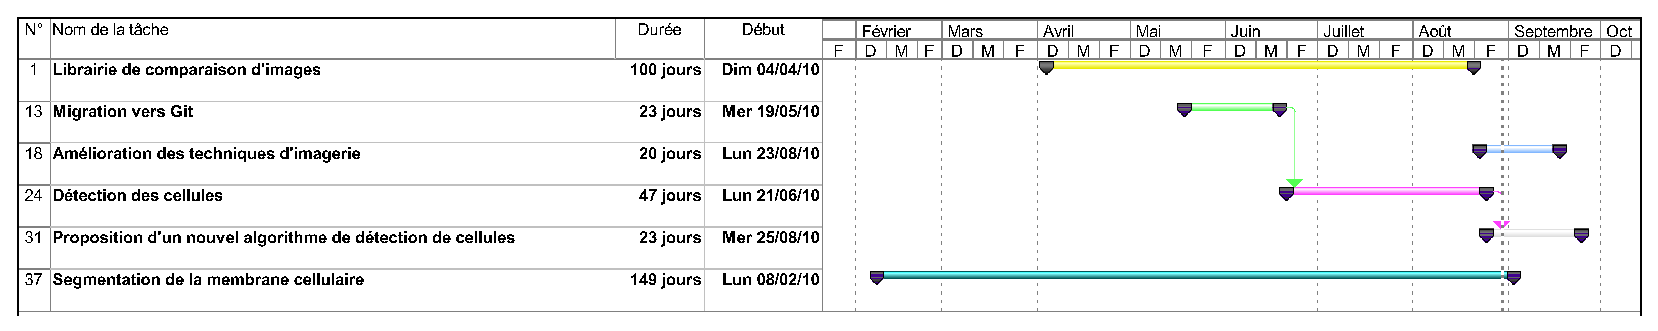
\includegraphics[ width=0.7\textheight, angle=-90,]{pictures/GanttPFE}
\end{center}
\caption{Gantt global du PFE}
\label{fig:GanttPFEGlobal}
\end{figure}
